
\section{Architecture Integration}

\subsection{Model Support}

\begin{table}[H]
\centering
\small
\begin{tabular}{lllll}
\toprule
\textbf{Architecture} & \textbf{Attention} & \textbf{RoPE?} & \textbf{GQA?} & \textbf{Verified} \\
\midrule
DistilBERT \& Flat \& No \& No &  \\
RoBERTa \& Nested \& No \& No &  \\
GPT-2 \& Causal \& No \& No &  \\
Qwen3.5 \& Causal + RoPE \& Yes \& Yes \& not tested \\
\bottomrule
\end{tabular}
\end{table}

\subsection{Weight Transfer}

\subsubsection{DistilBERT (Flat)}

\begin{lstlisting}
q\_lin, k\_lin, v\_lin, out\_lin
\end{lstlisting}

Direct copy with head-dim slicing. \texttt{is\_nested\_encoder = False}.

\subsubsection{RoBERTa (Nested)}

\begin{lstlisting}
attention.self.query, attention.self.key, attention.self.value
attention.output.dense
\end{lstlisting}

Extract from inner \texttt{self}. \texttt{is\_nested\_encoder = True}; skip own \texttt{out\_proj}.

\subsubsection{GPT-2 (Causal)}

\begin{lstlisting}
c\_attn (fused), c\_proj
\end{lstlisting}

Split fused \texttt{c\_attn}:

\begin{lstlisting}
w = src.c\_attn.weight.t()  # Conv1D transpose
q\_w, k\_w, v\_w = w.chunk(3, dim=0)
\end{lstlisting}

\subsubsection{Qwen3.5 (GQA + RoPE)}

GQA with pooling:

\begin{lstlisting}
if w\_k.shape[0] \textgreater{} self.kv\_head\_size:
    rep = w\_k.shape[0] // self.kv\_head\_size
    w\_k\_pooled = w\_k.view(self.num\_kv\_heads, rep, self.head\_dim, -1).mean(dim=1)
\end{lstlisting}

\subsection{Handling Nested Encoders}

For RoBERTa/BERT, \texttt{is\_nested\_encoder = True}:
\begin{itemize}
\item No \texttt{out\_proj} applied inside Squeezing Heads.
\item Outer \texttt{attention.output.dense} applies output.

\end{itemize}
\subsection{Causality}

Standard causal masking in forward:

\begin{lstlisting}
causal\_mask = torch.triu(torch.full((L, L), -inf), diagonal=1)
scores = scores + causal\_mask
\end{lstlisting}

\subsection{GQA Handling}

For Qwen/LLaMA with $H_{kv} < H$, use \texttt{repeat\_kv}:

\begin{lstlisting}
if self.num\_kv\_heads \textless{} self.num\_heads:
    k = repeat\_kv(k, self.kv\_repeat)
    v = repeat\_kv(v, self.kv\_repeat)
\end{lstlisting}

\subsection{Head-Dim Reduction}

If the target head\_dim $d_h' < d_h$, slice the leading rows of $W_Q, W_K, W_V$ 
and leading columns of $W_O$:

\begin{lstlisting}
m\_q\_out = min(self.q\_head\_size, w\_q.shape[0])  # = d\_h' * H
self.q\_proj.weight[:m\_q\_out, :m\_q\_in].copy\_(w\_q[:m\_q\_out, :m\_q\_in])
\end{lstlisting}

\subsection{Injection Algorithm}

\textbf{Algorithm 3:} Inject Squeezing Heads
\begin{lstlisting}
Input:  model M, config c
Output: M with LoRA-wrapped attention

1:  for   in transformer\_layers(M) do
2:      src $\leftarrow$ extract\_attention( )
3:      if src is None: continue
4:      new $\leftarrow$ SqueezingHeadsDistiller(config=c, old\_attn=src)
5:      replace\_attention( , new)
6: end for
\end{lstlisting}

\subsection{Failure Handling}

\texttt{inject\_squeezing\_heads} returns \texttt{None} on failure:

\begin{lstlisting}
try:
    new\_attn = SqueezingHeadsDistiller(...)
except Exception as e:
    logger.error("Failed to instantiate at layer \%d: \%s", layer\_idx, e)
    return None
\end{lstlisting}

\subsection{Parameter Count}

\begin{table}[H]
\centering
\small
\begin{tabular}{lll}
\toprule
\textbf{Component} & \textbf{Baseline} & \textbf{Squeezing Heads} \\
\midrule
Frozen $W_Q, W_K, W_V, W_O$ & $4 d^2$ & $4 d^2$ (same) \\
LoRA adapters & 0 & $4 r_L d$ \\
\textbf{Trainable} & $4 d^2$ & \textbf{$4 r_L d$} \\
\bottomrule
\end{tabular}
\end{table}

\subsection{Registry}

\begin{lstlisting}
@ATTENTION\_REGISTRY.register("squeezing\_heads")
@ATTENTION\_REGISTRY.register("squeezing\_heads\_distiller")
class SqueezingHeadsDistiller(BaseAttention): ...
\end{lstlisting}

\subsection{Failure Modes}

\begin{lstlisting}

---
\end{lstlisting}

\begin{figure}[H]
\centering
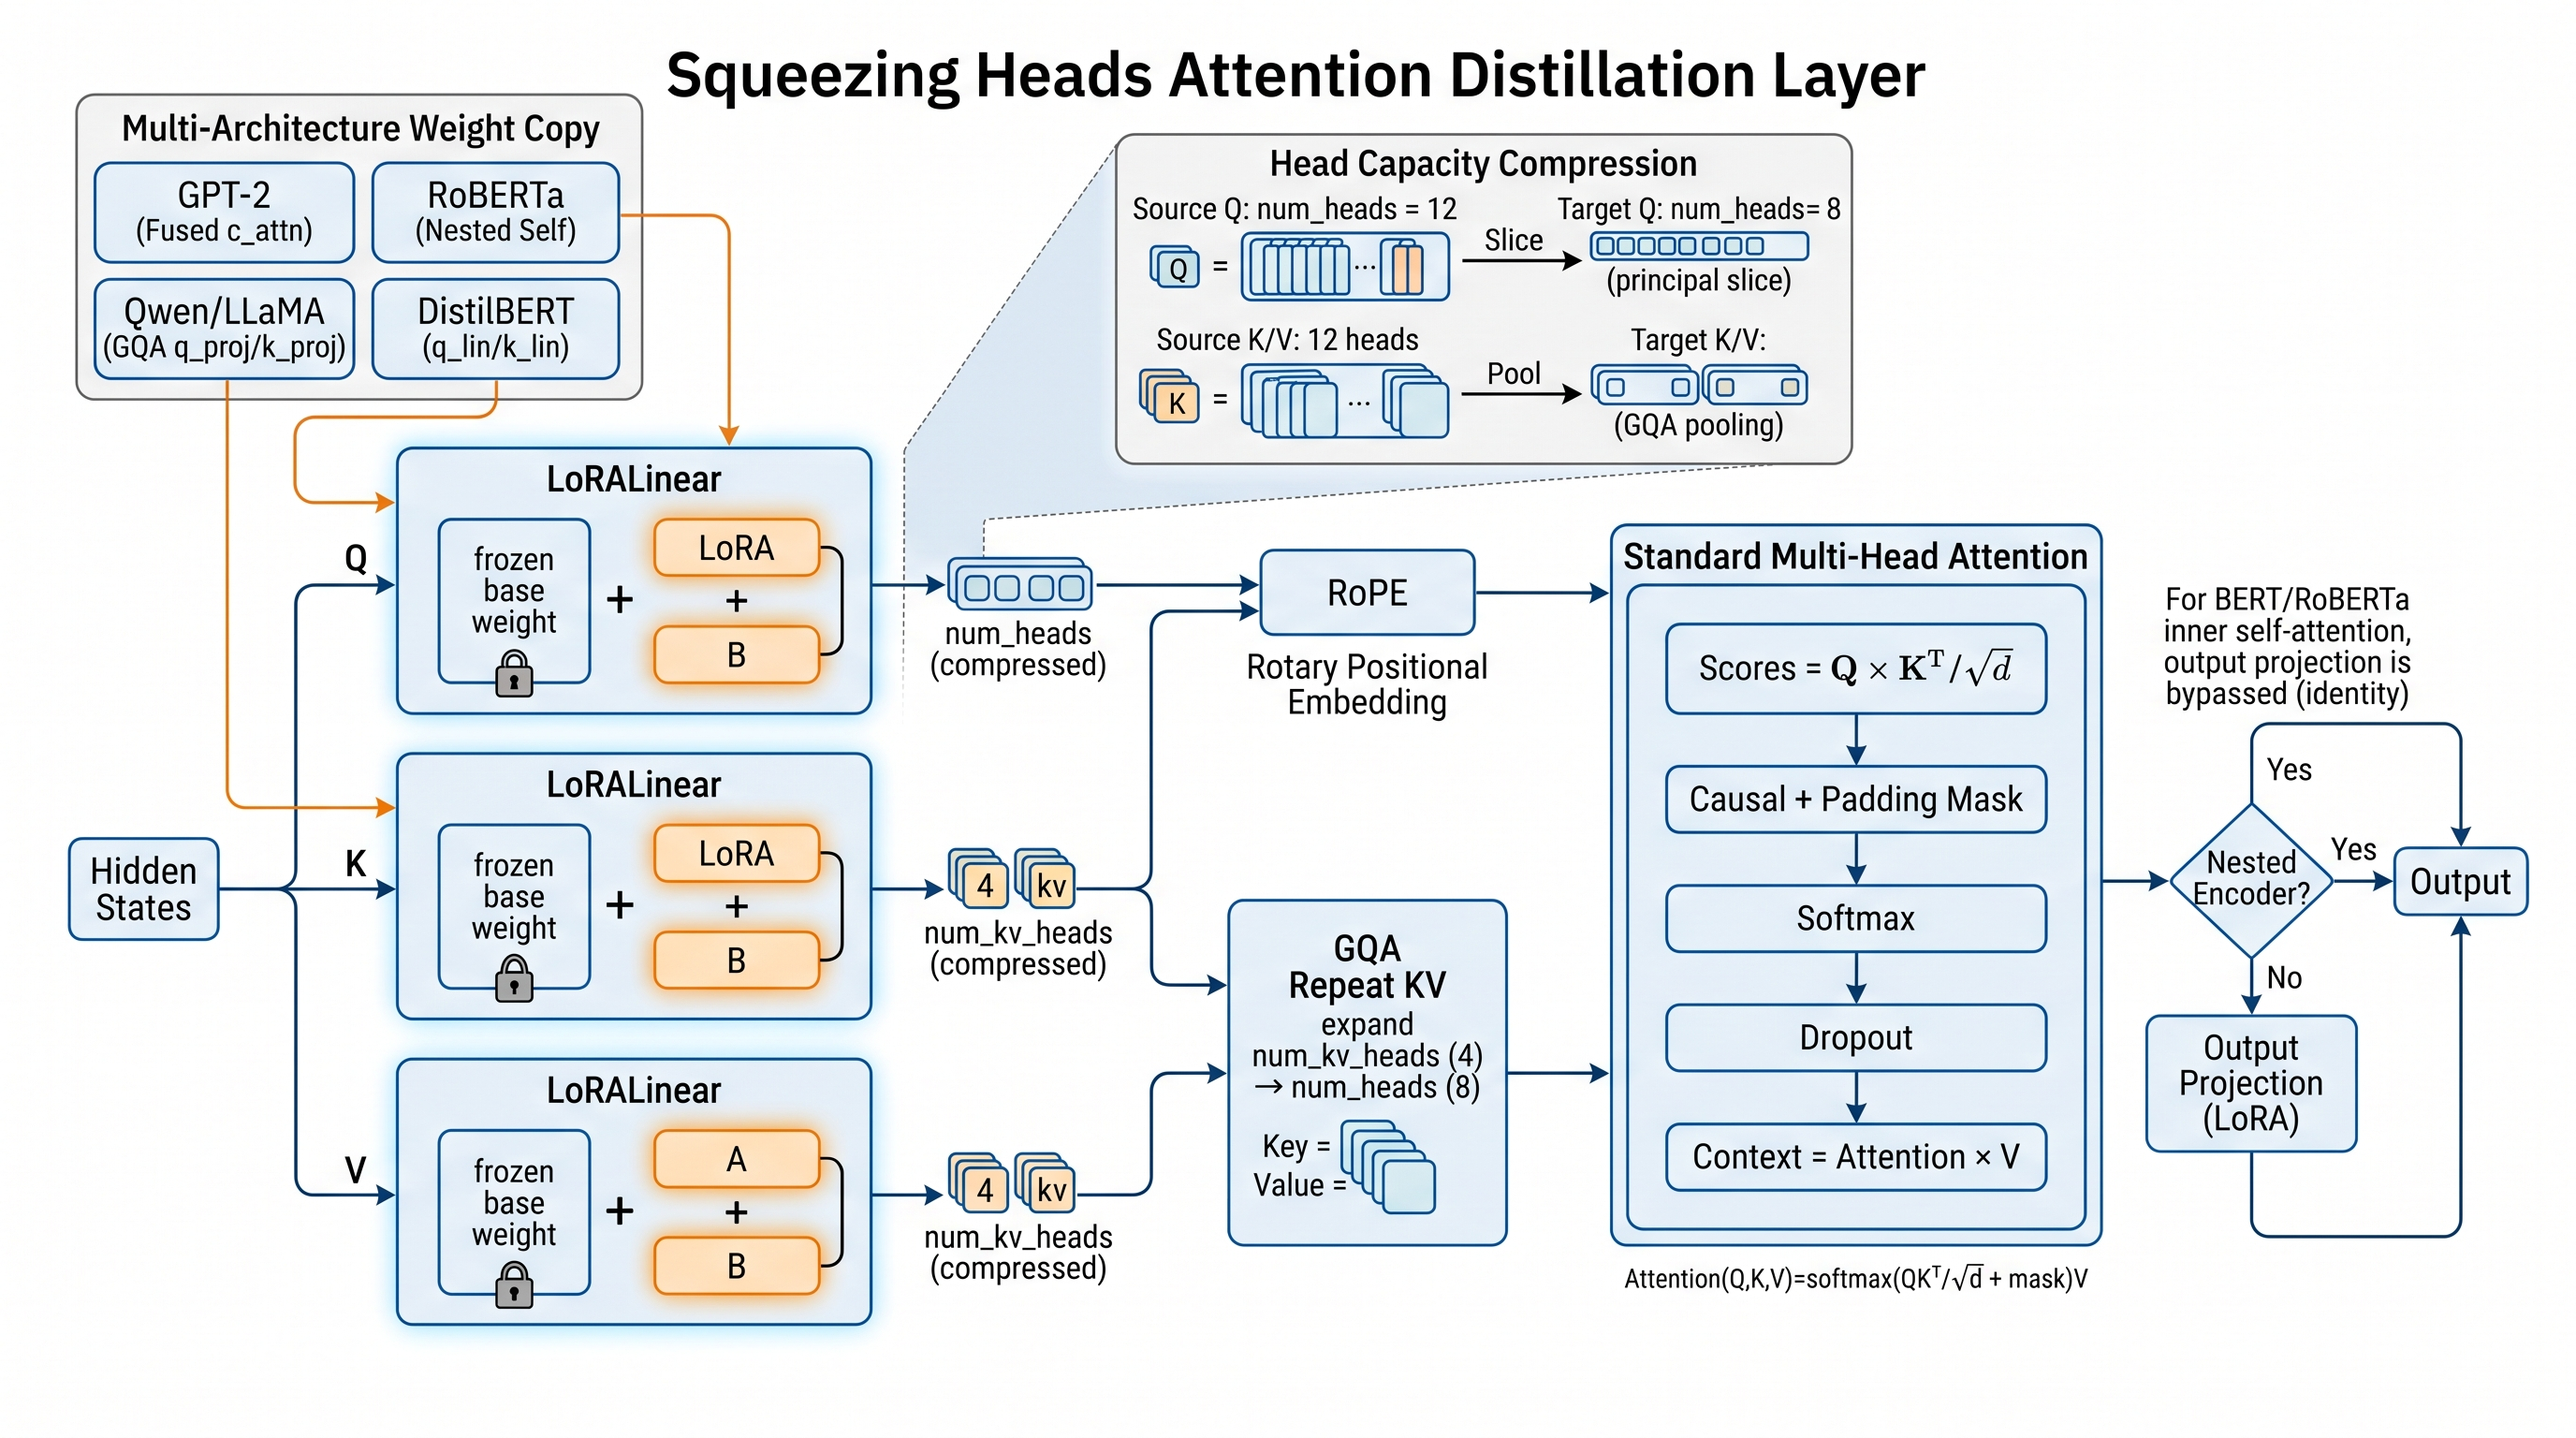
\includegraphics[width=\linewidth]{figures/architecture.jpeg}
\caption{High-level architectural diagram of SqueezingHeadsAttentionDistillationLayer.}
\label{fig:arch_SqueezingHeadsAttentionDistillationLayer}
\end{figure}

